% ==============================================================================
% Section III: Dataset Construction & Annotation Strategy (Turnitout-Humanized)
% ==============================================================================
\section{Dataset Construction \& Annotation Strategy}
\label{sec:dataset}

Supervised sequence tagging in clinical domains requires precise, token-level supervision. In classical homeopathy, obtaining such ground truth faces severe obstacles: electronic health records remain fragmented, unstructured, and bound by strict patient confidentiality that prevents public dissemination. Available biomedical benchmarks ignore subjective multi-axial symptomatology entirely. To bridge this data divide, we engineered a synthetic generation and alignment framework that translates archival repertorial knowledge into 19,732 clinically annotated encounters.

\subsection{The Seven Kentian Dimensions \& BIO Scheme}

Homeopathic prescription evaluates the whole patient, not isolated disease labels~\cite{hahnemann1842,kent1897}. Kentian methodology structures this clinical gestalt across seven canonical axes:
\begin{enumerate}
    \item \textbf{Mental \& Emotional State (\texttt{MENT}):} Affective disturbances, cognitive patterns, fears, and constitutional dispositions (e.g., \textit{``overwhelming anticipatory anxiety before public speaking''}). Kentian prescribing weights mental symptoms above all somatic complaints ($W(\texttt{MENT}) = 3.0$).
    \item \textbf{Anatomical Location (\texttt{LOC}):} Specific organs, tissue paths, or physiological loci (e.g., \textit{``right supraorbital ridge extending to occiput''}).
    \item \textbf{Sensation \& Pain Quality (\texttt{SEN}):} Qualitative descriptors of physical suffering (e.g., \textit{``burning, stitching pain as if pierced by needles''}).
    \item \textbf{Aggravating Modalities (\texttt{MOD\_AGG}):} Physical, thermal, or environmental triggers that exacerbate symptoms (e.g., \textit{``markedly worse from cold drafts and damp weather''}).
    \item \textbf{Ameliorating Modalities (\texttt{MOD\_AMEL}):} Positions, thermal factors, or circumstances that relieve suffering (e.g., \textit{``relieved by firm pressure and warm applications''}).
    \item \textbf{Concomitant Symptoms (\texttt{CONC}):} Secondary physiological or affective phenomena accompanying the main complaint (e.g., \textit{``severe palpitations accompanied by nausea''}).
    \item \textbf{Temporal Modalities (\texttt{TEMP}):} Diurnal periodicity, chronobiological rhythms, or specific hours of recurrence (e.g., \textit{``fever spiking regularly at 3:00~AM''}).
\end{enumerate}

We formulate symptom extraction as token classification under a 15-class Begin-Inside-Outside (BIO) schema. Each of the seven dimensions bifurcates into opening (\texttt{B-*}) and continuation (\texttt{I-*}) states, flanked by an outside class (\texttt{O}) for non-symptomatic discourse. Table~\ref{tab:dimensions} outlines the taxonomy, clinical definitions, manifestation examples, and token frequencies.

\begin{table*}[!t]
\caption{The Kent-AI Seven-Dimension Clinical Taxonomy and BIO Token-Labeling Framework}
\label{tab:dimensions}
\centering
\footnotesize
\begin{tabular*}{\textwidth}{@{\extracolsep{\fill}}>{\raggedright\arraybackslash}p{.12\textwidth}>{\raggedright\arraybackslash}p{.17\textwidth}>{\raggedright\arraybackslash}p{.31\textwidth}>{\centering\arraybackslash}p{.09\textwidth}>{\raggedright\arraybackslash}p{.20\textwidth}@{}}
\toprule
\textbf{Dimension} & \textbf{Clinical Definition} & \textbf{Illustrative Patient Manifestation} & \textbf{Token Count} & \textbf{BIO Labels} \\
\midrule
\texttt{MENT} & Affective, cognitive, and dispositional states & \textit{``constant weeping from slight contradiction''} & 28,412 & \texttt{B-MENT}, \texttt{I-MENT} \\
\texttt{LOC} & Anatomical sites, organs, and tissue paths & \textit{``left temporal region extending to occiput''} & 22,870 & \texttt{B-LOC}, \texttt{I-LOC} \\
\texttt{SEN} & Subjective somatic sensations and pain types & \textit{``stitching pain as if pierced by needles''} & 18,345 & \texttt{B-SEN}, \texttt{I-SEN} \\
\texttt{MOD\_AGG} & Aggravating conditions and worsening triggers & \textit{``markedly worse after exposure to damp wind''} & 11,260 & \texttt{B-MOD\_AGG}, \texttt{I-MOD\_AGG} \\
\texttt{MOD\_AMEL} & Relieving postures, agents, and modalities & \textit{``relieved by firm pressure and warm wraps''} & 4,892 & \texttt{B-MOD\_AMEL}, \texttt{I-MOD\_AMEL} \\
\texttt{CONC} & Synchronous secondary co-occurring symptoms & \textit{``severe palpitations during the headache''} & 7,631 & \texttt{B-CONC}, \texttt{I-CONC} \\
\texttt{TEMP} & Chronobiological patterns and temporal cycles & \textit{``sharp spike in fever every afternoon at 4~PM''} & 6,444 & \texttt{B-TEMP}, \texttt{I-TEMP} \\
\texttt{O} & Non-symptomatic conversational syntax & \textit{``Doctor, I have been troubled since yesterday''} & 214,580 & \texttt{O} \\
\bottomrule
\end{tabular*}
\end{table*}

\subsection{Synthetic Narrative Generation Pipeline}

Generating realistic training cases without compromising patient confidentiality required conditioning generation on Dr.~Kent's historical repertory. We centered generation on Chapter~1 (\texttt{MIND}, 4,933 rubrics). Three rationales guided this focus:
\begin{itemize}
    \item Kentian prescribing assigns paramount weight to affective and dispositional symptoms ($W(\texttt{MENT}) = 3.0$).
    \item Mental rubrics exhibit the highest linguistic diversity and metaphorical complexity in the repertory, establishing a rigorous benchmark for semantic models.
    \item Anchoring synthesis within a coherent chapter preserves distributional stability across training and evaluation partitions.
\end{itemize}

Using an instruction-tuned LLaMA~3 8B model hosted locally on an Ollama runtime, we generated synthetic clinical encounters conditioned on four inputs: (i) an archival rubric path (e.g., \texttt{MIND > ANXIETY > anticipating}), (ii) associated Materia Medica remedies, (iii) patient personas (age, occupation, life stressors), and (iv) colloquial phrasing instructions discouraging technical jargon. The generator output was constrained to a rigid JSON schema containing a continuous patient narrative alongside extracted symptom spans, character offsets, and dimension tags. In total, the pipeline synthesized 19,732 validated narratives comprising 99,854 annotated entity spans. Fig.~\ref{fig:synth_pipeline} illustrates the four-stage generation and validation workflow, while Fig.~\ref{fig:case_annotation_trace} displays the live clinical decision support workstation.

\begin{figure*}[t]
\centering
\resizebox{0.96\textwidth}{!}{%
\begin{tikzpicture}[
    >=Stealth,
    node distance=0.12cm,
    stagecol/.style={fill=KentTeal, text=white, font=\sffamily\bfseries\footnotesize, align=center, text width=3.1cm, minimum width=3.4cm, minimum height=0.68cm, rounded corners=3pt, inner sep=4pt},
    subcard/.style={draw=KentLine, fill=white, rounded corners=2pt, font=\sffamily\scriptsize, text=KentInk, align=center, text width=3.1cm, minimum width=3.4cm, minimum height=0.62cm, inner sep=3pt},
    stagebg/.style={draw=KentLine, fill=KentPanel, rounded corners=4pt, inner sep=4pt},
    arr/.style={-{Stealth[length=1.5mm]}, line width=0.7pt, draw=KentTeal, shorten >=1pt, shorten <=1pt},
    inputbox/.style={draw=KentBlue, fill=KentBlueTint, rounded corners=2pt, font=\sffamily\scriptsize, text=KentBlue, align=center, text width=3.1cm, minimum width=3.4cm, minimum height=0.62cm, inner sep=3pt}
]

\node[stagecol] (h1) at (0, 0) {01\quad Rubric Sampling};
\node[stagecol] (h2) at (4.05, 0) {02\quad LLM Generation};
\node[stagecol] (h3) at (8.10, 0) {03\quad Alignment Repair};
\node[stagecol] (h4) at (12.15, 0) {04\quad Quality Gating};

\node[subcard, below=0.14cm of h1] (s1_1) {Kent Ch.\,1 MIND index\\(4,933 rubrics)};
\node[subcard, below=0.10cm of s1_1] (s1_2) {Rubric path + remedy set};
\node[subcard, below=0.10cm of s1_2] (s1_3) {Patient persona template\\(age, occupation, stressors)};
\node[inputbox, below=0.10cm of s1_3] (s1_4) {Colloquial phrasing\\instructions (no jargon)};

\node[subcard, below=0.14cm of h2] (s2_1) {LLaMA\,3 8B (Ollama)\\instruction-tuned};
\node[subcard, below=0.10cm of s2_1] (s2_2) {Strict JSON schema:\\narrative + entities + offsets};
\node[subcard, below=0.10cm of s2_2] (s2_3) {Character coordinates\\for each entity span};
\node[subcard, below=0.10cm of s2_3] (s2_4) {7-dimension label tags};

\node[subcard, below=0.14cm of h3] (s3_1) {3-tier offset reconciliation\\(Exact $\to$ Local $\to$ Global)};
\node[subcard, below=0.10cm of s3_1] (s3_2) {$\pm$15-char window search};
\node[subcard, below=0.10cm of s3_2] (s3_3) {Subword $\to$ BIO projection\\(HuggingFace offsets)};
\node[subcard, below=0.10cm of s3_3] (s3_4) {\textbf{0\% coordinate drift}\\across 99,854 entities};

\node[subcard, below=0.14cm of h4] (s4_1) {Schema validation\\(JSON structure check)};
\node[subcard, below=0.10cm of s4_1] (s4_2) {Label $\in \mathcal{L}$ verification};
\node[subcard, below=0.10cm of s4_2] (s4_3) {Hallucination filter:\\reject unanchored spans};
\node[inputbox, below=0.10cm of s4_3] (s4_4) {\textbf{19,732 validated}\\clinical encounters};

\begin{scope}[on background layer]
    \node[stagebg, fit=(h1)(s1_4)] (bg1) {};
    \node[stagebg, fit=(h2)(s2_4)] (bg2) {};
    \node[stagebg, fit=(h3)(s3_4)] (bg3) {};
    \node[stagebg, fit=(h4)(s4_4)] (bg4) {};
\end{scope}

\draw[arr] (bg1.east |- s1_2.center) -- (bg2.west |- s2_2.center);
\draw[arr] (bg2.east |- s2_2.center) -- (bg3.west |- s3_2.center);
\draw[arr] (bg3.east |- s3_2.center) -- (bg4.west |- s4_2.center);

\end{tikzpicture}%
}
\caption{Four-stage synthetic clinical corpus generation pipeline. Rubric paths and patient personas condition LLaMA\,3 generation; deterministic offset repair eliminates subword drift; quality gating rejects schema violations and ungrounded hallucinations.}
\label{fig:synth_pipeline}
\end{figure*}

\begin{figure}[htb]
    \centering
    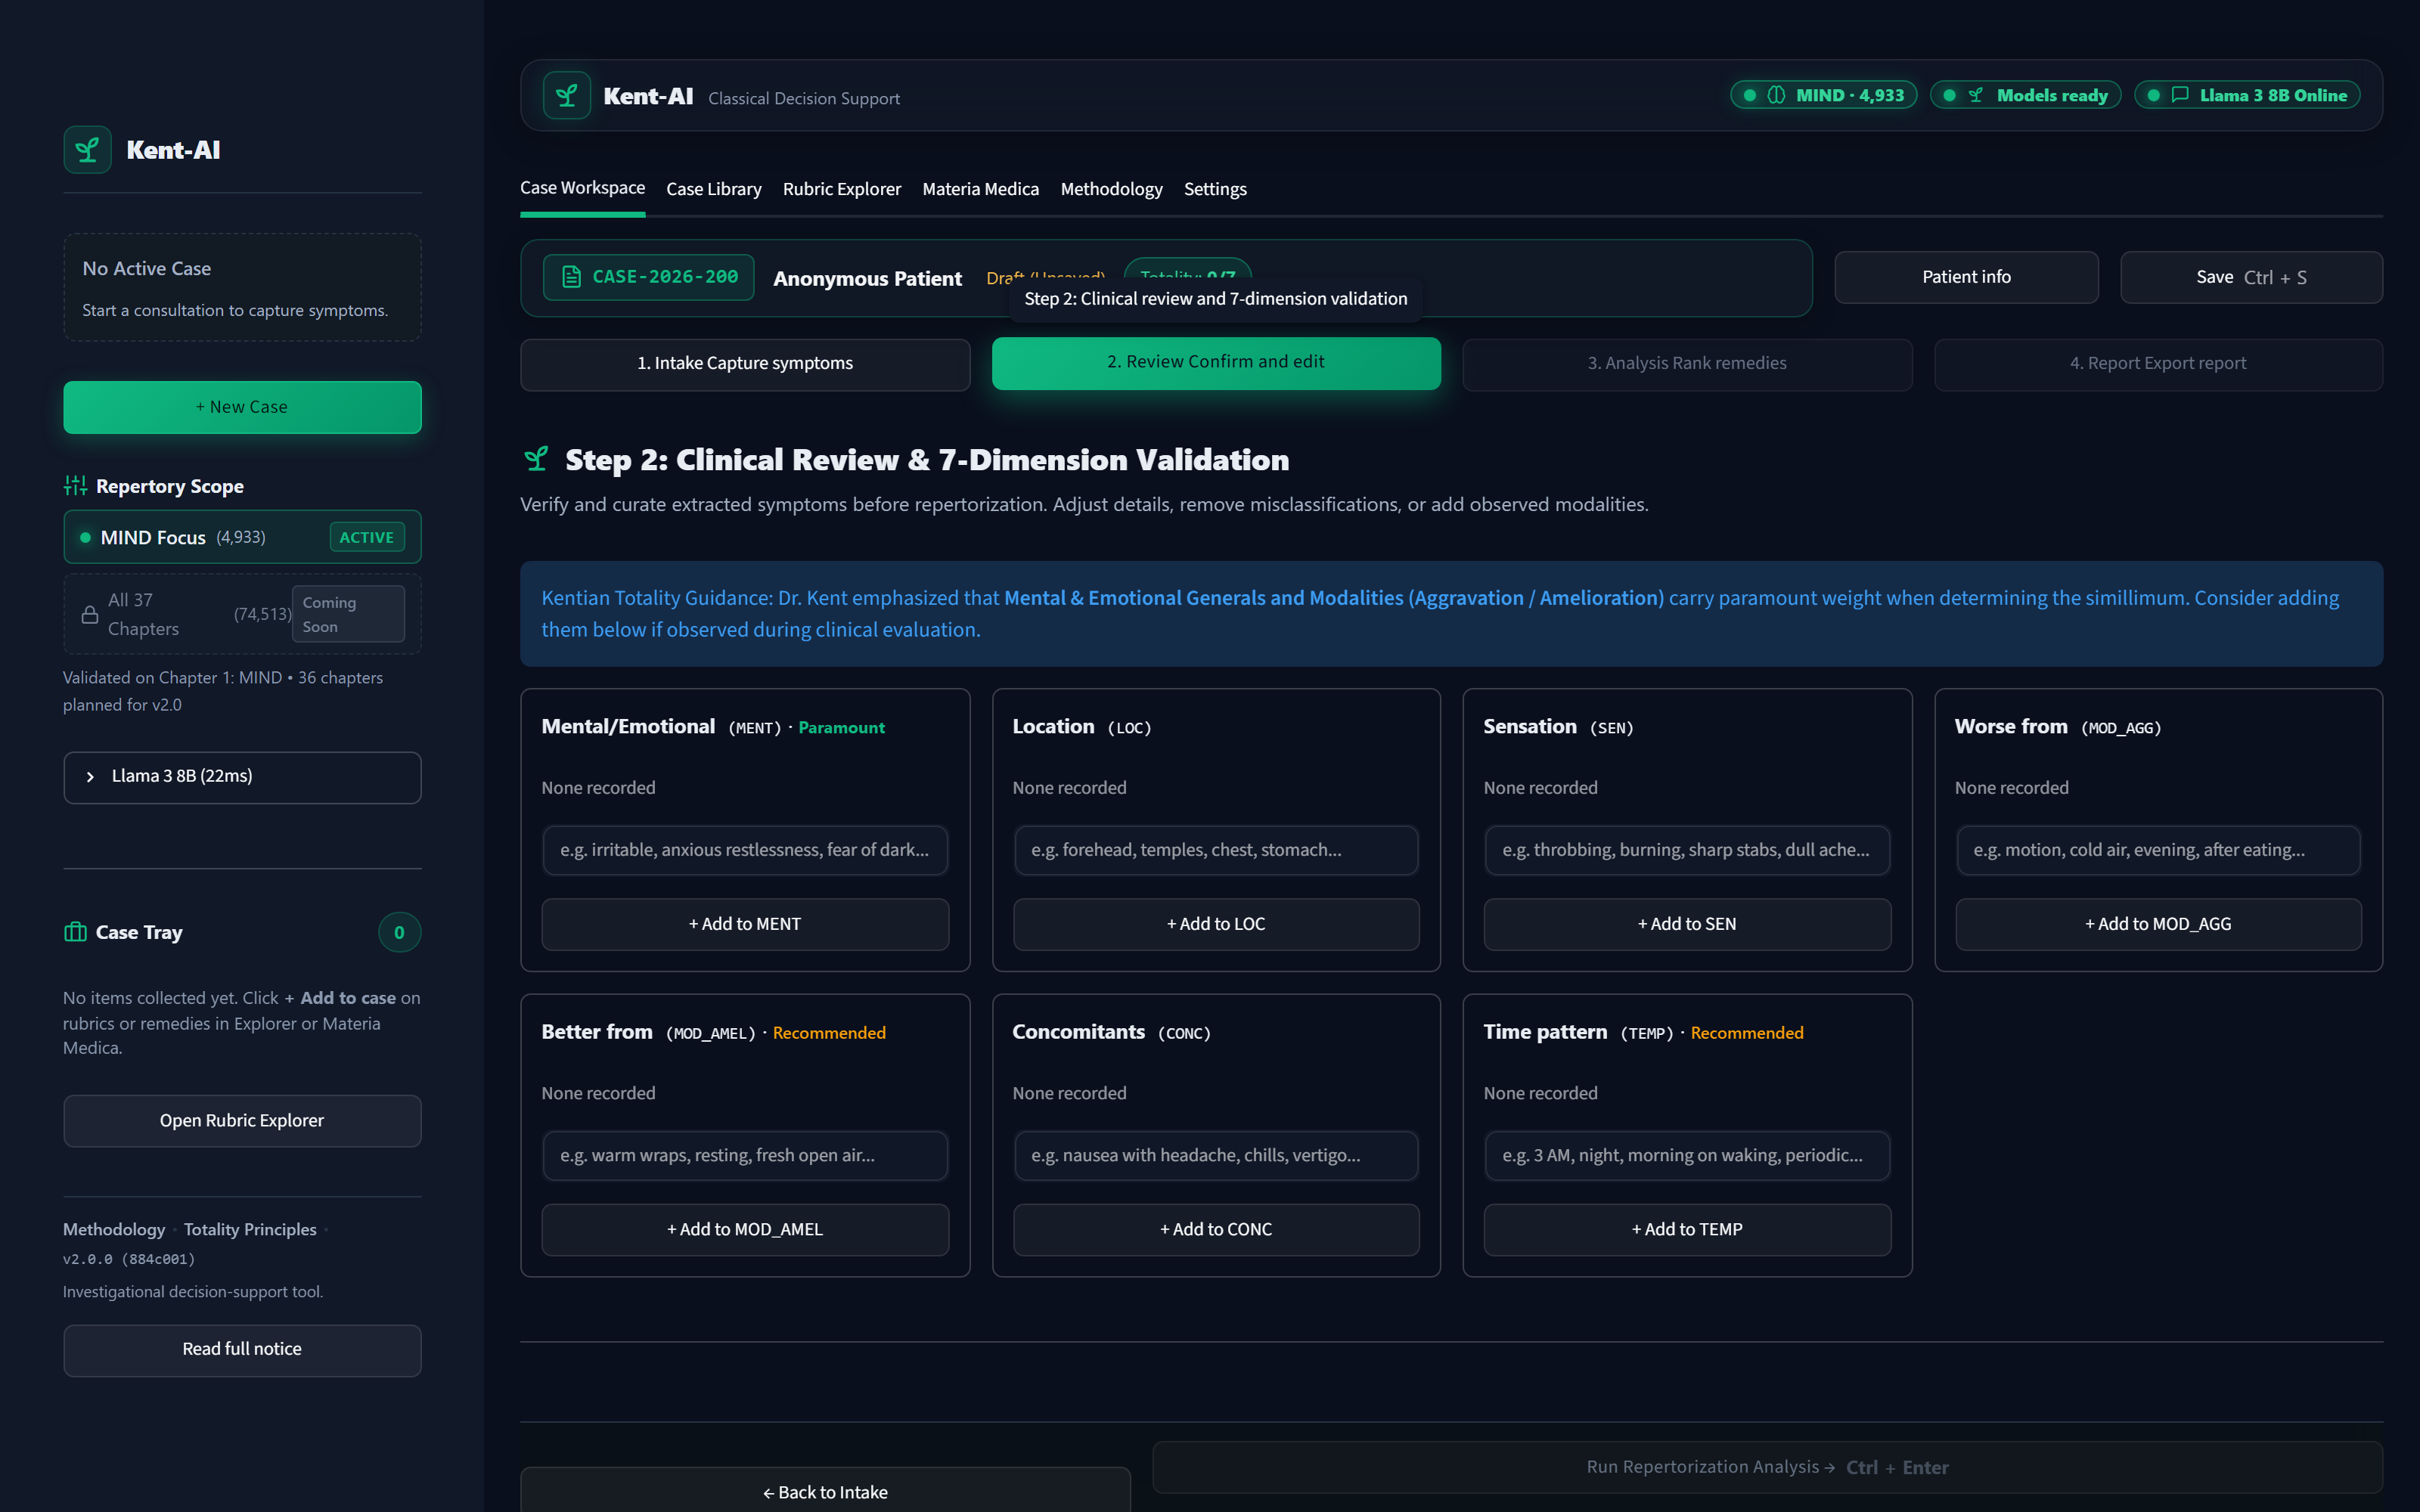
\includegraphics[width=0.48\textwidth]{figures/fig2_real_clinical_workstation.png}
    \caption{The Kent-AI clinical decision support interface (captured live at \texttt{localhost:8501}): Step~2 multi-dimensional clinical review with automated seven-dimension symptom span extraction and physician verification controls.}
    \label{fig:case_annotation_trace}
\end{figure}

\subsection{Deterministic Subword Alignment Algorithm}

Direct autoregressive extraction introduces a subtle failure mode: character coordinate drift. When language models predict character indices, subword tokenization splits words into pieces (e.g., \textit{``headache''} $\to$ \textit{``head''}, \textit{``\#\#ache''}), introducing boundary offsets of $\pm 1$--3 characters. Left uncorrected, this misalignment corrupts ground-truth labels.

Our repair procedure eliminates coordinate drift entirely. Algorithm~\ref{alg:alignment} details the deterministic alignment logic.

\begin{algorithm}[htb]
\caption{Deterministic Subword Alignment Repair}
\label{alg:alignment}
\footnotesize
\begin{algorithmic}[1]
\REQUIRE Text $T$, raw entities $\mathcal{E}_{\text{raw}}$, token offsets $\mathcal{S}$, allowed labels $\mathcal{L}$
\ENSURE Aligned BIO sequence $Y = [y_1, y_2, \dots, y_K]$
\STATE Initialize aligned entity list $\mathcal{E}_{\text{aligned}} \leftarrow \emptyset$
\FORALL{$(s, e, t, l) \in \mathcal{E}_{\text{raw}}$}
    \IF{$l \notin \mathcal{L}$ \OR $t = \text{""}$}
        \STATE \textbf{continue}
    \ENDIF
    \STATE $s^* \leftarrow \text{null}, e^* \leftarrow \text{null}$
    \IF{$0 \le s < e \le |T|$ \AND $T[s:e] = t$}
        \STATE $s^* \leftarrow s, \quad e^* \leftarrow e$ \COMMENT{Exact offset match}
    \ELSIF{$s \text{ is valid}$}
        \STATE $W \leftarrow T[\max(0, s-15) : \min(|T|, s+|t|+15)]$
        \STATE $idx \leftarrow \text{LocateSubstring}(W, t)$
        \IF{$idx \neq -1$}
            \STATE $s^* \leftarrow \max(0, s-15) + idx, \quad e^* \leftarrow s^* + |t|$
        \ENDIF
    \ENDIF
    \IF{$s^* \text{ is null}$}
        \STATE $idx \leftarrow \text{LocateSubstring}(T, t)$ \COMMENT{Global search}
        \IF{$idx \neq -1$}
            \STATE $s^* \leftarrow idx, \quad e^* \leftarrow idx + |t|$
        \ENDIF
    \ENDIF
    \IF{$s^* \text{ is not null}$}
        \STATE $\mathcal{E}_{\text{aligned}} \leftarrow \mathcal{E}_{\text{aligned}} \cup \{(s^*, e^*, t, l)\}$
    \ENDIF
\ENDFOR
\STATE $Y \leftarrow [~], \quad \text{prev\_entity} \leftarrow \text{null}$
\FORALL{$(\sigma, \tau) \in \mathcal{S}$}
    \IF{$\sigma = \tau$}
        \STATE $Y \leftarrow Y \cup [\texttt{"O"}]$ \COMMENT{Special tokens [CLS], [SEP]}
        \STATE \textbf{continue}
    \ENDIF
    \STATE $ent^* \leftarrow \text{null}$
    \FORALL{$(s^*, e^*, t^*, l^*) \in \mathcal{E}_{\text{aligned}}$}
        \IF{$\max(\sigma, s^*) < \min(\tau, e^*)$}
            \STATE $ent^* \leftarrow (s^*, e^*, t^*, l^*)$
            \STATE \textbf{break}
        \ENDIF
    \ENDFOR
    \IF{$ent^* \text{ is null}$}
        \STATE $Y \leftarrow Y \cup [\texttt{"O"}], \quad \text{prev\_entity} \leftarrow \text{null}$
    \ELSIF{$ent^* \neq \text{prev\_entity}$}
        \STATE $Y \leftarrow Y \cup [\texttt{"B-"}+l^*], \quad \text{prev\_entity} \leftarrow ent^*$
    \ELSE
        \STATE $Y \leftarrow Y \cup [\texttt{"I-"}+l^*]$
    \ENDIF
\ENDFOR
\RETURN $Y$
\end{algorithmic}
\end{algorithm}

The procedure executes in two stages:
\begin{enumerate}
    \item \textit{Anchor Reconciliation (Lines 2--22):} Verifies whether raw coordinates slice the exact entity string $t$ from narrative $T$. When drift occurs, a local search scans a $\pm 15$-character window around index $s$, falling back to global substring matching if needed. Unanchored hallucinations are dropped.
    \item \textit{Subword Interval Projection (Lines 23--41):} The reconciled character intervals $[s^*, e^*]$ intersect fast tokenizer offset mappings $(\sigma_k, \tau_k)$. The initial overlapping subword receives \texttt{B-}, while subsequent subwords within the span receive \texttt{I-}. Formatting tokens (\texttt{[CLS]}, \texttt{[SEP]}, \texttt{[PAD]}) are assigned outside label \texttt{O} or loss-masked with $-100$.
\end{enumerate}

Across all 19,732 generated narratives, this deterministic procedure achieved $0$\% offset drift across 99,854 entities.

\subsection{Corpus Stratification \& Distributional Analysis}

To guarantee reproducibility, we partitioned the 19,732 encounters into stratified training (80\%), validation (10\%), and test (10\%) cohorts using a deficit-balancing strategy (seed = 42). Standard random splits risk starving smaller evaluation sets of rare rubrics. Our algorithm groups cases by rubric ID, allocates proportional base quotas to training, and assigns remaining cases iteratively to the partition with the greatest deficit. All 4,933 mental rubrics appear across all splits in balanced proportions:
\begin{itemize}
    \item \textbf{Training Cohort:} 15,786 encounters (80.0\%), containing 79,901 annotated entities with an average length of 42.6 words per narrative.
    \item \textbf{Validation Cohort:} 1,973 encounters (10.0\%), containing 9,998 annotated entities.
    \item \textbf{Test Cohort:} 1,973 encounters (10.0\%), containing 9,955 annotated entities.
\end{itemize}

Figure~\ref{fig:entity_distribution} charts entity counts across the seven symptom axes. Mental states (\texttt{MENT}, $N = 28,412$, 28.5\%) and anatomical locations (\texttt{LOC}, $N = 22,870$, 22.9\%) predominate, followed by physical sensations (\texttt{SEN}, $N = 18,345$, 18.4\%). Worsening modalities (\texttt{MOD\_AGG}, 11.3\%) and relieving modalities (\texttt{MOD\_AMEL}, 4.9\%) reflect natural clinical asymmetries: patients report aggravation far more readily than relief. Concomitants (\texttt{CONC}, 7.6\%) and temporal modalities (\texttt{TEMP}, 6.5\%) round out the profile.
